% =============================================================================

\vspace*{\fill}

\begin{figure}[!h]
\begin{lstlisting}[language=pseudo,style=block]
saes.v2.encs rd, rs1, rs2 : v2.SubBytes(rd, rs1, rs2, fwd=1)
saes.v2.decs rd, rs1, rs2 : v2.SubBytes(rd, rs1, rs2, fwd=0)
saes.v2.encm rd, rs1, rs2 : v2.MixColumns(rd, rs1, rs2, fwd=1)
saes.v2.decm rd, rs1, rs2 : v2.MixColumns(rd, rs1, rs2, fwd=0)
\end{lstlisting}
\caption{
  Instruction mnemonics, and their mapping onto pseudo-code functions, for \ISE{2}.
}
\label{fig:v2:mnemonics}
\end{figure}

\begin{figure}[!h]
\begin{lstlisting}[language=pseudo,style=block]
v2.SubBytes(rd, rs1, rs2, fwd):
  t1.32  = {rs1.8[0], rs2.8[1], rs1.8[2], rs2.8[3]}
  rd.8[i]= AESSBox[t1.8[i]] if fwd else AESInvSBox[t1.8[i]] for i=0..3

v2.MixColumns(rd, rs1, rs2, fwd):
  t1.32  = {rs1.8[0], rs1.8[1], rs2.8[2], rs2.8[3]}
  for i=0..3:
      tmp.32 = ROTL32(rs1.32, 8*i)
      rd.8[i]= AESMixColumn(tmp.32) if fwd else AESInvMixColumn(tmp.32)
\end{lstlisting}
\caption{
  Instruction pseudo-code functions for \ISE{2}.
}
\label{fig:v2:pseudo}
\end{figure}

\begin{figure}[!h]
\begin{lstlisting}[language=pseudo,style=block]
lw              a0,  0(a4)     // Load Round Key
lw              a1,  4(a4)
lw              a2,  8(a4)
lw              a3, 12(a4)
xor             t0, t0, a0     // Add Round Key
xor             t1, t1, a1
xor             t2, t2, a2
xor             t3, t3, a3
saes.v2.sub.enc a0, t0, t1     // SubBytes / ShiftRows
saes.v2.sub.enc a1, t2, t3
saes.v2.sub.enc a2, t1, t2
saes.v2.sub.enc a3, t3, t0
saes.v2.mix.enc t0, a0, a1     // ShiftRows / MixColumns
saes.v2.mix.enc t1, a2, a3
saes.v2.mix.enc t2, a1, a0
saes.v2.mix.enc t3, a3, a2
\end{lstlisting}
\caption{
  An AES encryption round implemented using \ISE{2}.
}
\label{fig:v2:round}
\end{figure}

\vspace*{\fill}

% -----------------------------------------------------------------------------

\newpage

\vspace*{\fill}

\begin{figure}[!h]
\centering
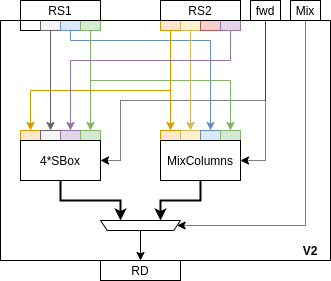
\includegraphics[width={0.5\textwidth}]{diagrams/ise-datapath-v2.png}
\caption{
  A diagrammatic description of the functional unit required to support \ISE{2}.
}
\label{fig:v2:fu}
\end{figure}

\vspace*{\fill}

% =============================================================================
